\documentclass[border=8pt]{standalone}
\usepackage{tikz}
\usetikzlibrary{positioning, fit, arrows.meta, calc}

\begin{document}

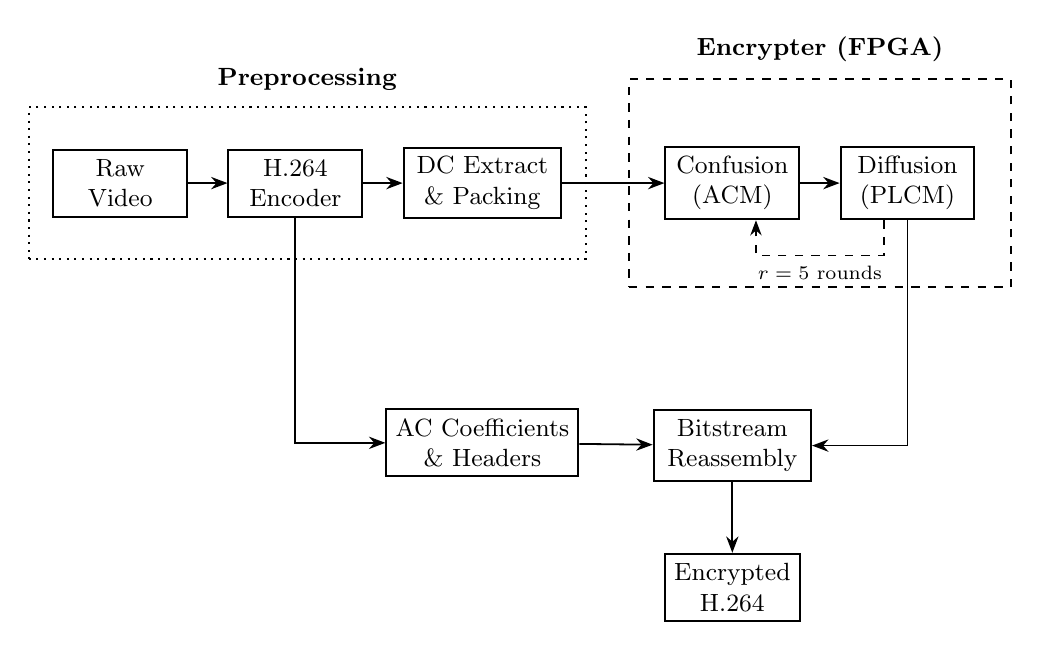
\begin{tikzpicture}[
    >=Stealth,
    font=\small,
    node distance=0.55cm and 0.5cm,
    block/.style={
        rectangle, draw, line width=0.7pt,
        minimum width=1.7cm, minimum height=0.85cm,
        align=center, fill=white
    },
    blockW/.style={
        rectangle, draw, line width=0.7pt,
        minimum width=2.0cm, minimum height=0.85cm,
        align=center, fill=white
    },
    arrow/.style={->, line width=0.65pt},
    dasharrow/.style={->, line width=0.55pt, dashed}
]

%% ─── ROW 1: encryption flow ─────────────────────────────────────────────

\node[block]                       (raw)    {Raw\\Video};
\node[block, right=of raw]         (h264)   {H.264\\Encoder};
\node[blockW, right=of h264]       (pack)   {DC Extract\\$\&$ Packing};

\node[block, right=1.3cm of pack]  (acm)    {Confusion\\(ACM)};
\node[block, right=of acm]         (plcm)   {Diffusion\\(PLCM)};

%% ─── ROW 2: AC buffer + Reassembly ──────────────────────────────────────

\node[blockW, below=2.4cm of pack] (ac)     {AC Coefficients\\$\&$ Headers};

\node[blockW, below=2.4cm of acm]  (reasm)  {Bitstream\\Reassembly};

%% ─── ROW 3: Encrypted output ────────────────────────────────────────────

\node[block, below=0.9cm of reasm] (out)    {Encrypted\\H.264};

%% ─── ROW 1 ARROWS ────────────────────────────────────────────────────────

\draw[arrow] (raw)   -- (h264);
\draw[arrow] (h264)  -- (pack);
\draw[arrow] (pack)  -- (acm);
\draw[arrow] (acm)   -- (plcm);

%% ─── ROW 2 ARROWS ────────────────────────────────────────────────────────

\draw[arrow] (ac)    -- (reasm);

%% ─── CROSS-ROW LINKS ────────────────────────────────────────────────────

% H264 Encoder → AC buffer (down then left)
\draw[arrow] (h264.south) |- (ac.west);

% Diffusion → Reassembly (down + left to reach east side)
\draw[arrow] (plcm.south) |- (reasm.east);

% Reassembly → Encrypted H.264 (down)
\draw[arrow] (reasm) -- (out);

%% ─── ROUND LOOP (dashed, BELOW the two blocks but INSIDE box) ───────────

\draw[dasharrow]
    ($(plcm.south)+(-0.3,0)$) -- ++(0,-0.45)
    -- node[below, font=\scriptsize] {$r = 5$ rounds}
    ($(acm.south)+(0.3,-0.45)$) -- ($(acm.south)+(0.3,0)$);

%% ─── ENCRYPTER (FPGA) BOUNDARY ───────────────────────────────────────────

\node[
    rectangle, draw, dashed, line width=0.8pt,
    inner xsep=0.45cm, inner ysep=0.85cm,
    fit=(acm)(plcm)
] (encbox) {};

\node[above=0.08cm of encbox, font=\small\bfseries] 
    {Encrypter (FPGA)};

%% ─── PREPROCESSING BOUNDARY ──────────────────────────────────────────────

\node[
    rectangle, draw, dotted, line width=0.75pt,
    inner xsep=0.3cm, inner ysep=0.5cm,
    fit=(raw)(h264)(pack)
] (prepbox) {};

\node[above=0.08cm of prepbox, font=\small\bfseries]
    {Preprocessing};

\end{tikzpicture}

\end{document}
